\chapter{A construção do painel}\label{cap_trabalho_academico}

Antes de avançar para a parte técnica, é importante explicar o que é o Centro de Inteligência da JFRN e como um painel poderia ajudar na tarefa deles.

De acordo com o site do Centro de Inteligência, ele existe para otimizar o trabalho jurisdicional a partir de demandas repetitivas. Esse tipo de demanda deve ser comunicado às autoridades para que a multiplicação desses casos diminuam, e não haja uma sobrecarga. Portanto, o painel será usado para auxiliar na análise dessas demandas, tentando acompanhar a evolução e desenvolvimento delas, agindo para que elas não sobrecarreguem a JFRN.


\section{Python}

Python é uma linguagem de programação de alto nível e de aplicações gerais, foi criada por Guido van Rossum e lançada em 1991. Suporta vários paradigmas, incluindo orientação a objeto e programação funcional. Essas características a tornaram muito popular entre programadores, porque é possível construir muita coisa usando poucas linhas de código, e esses projetos vão desde um timer simples, até grandes análises de dados e sistemas com inteligência artificial.

No final do capítulo 1 foram detalhadas algumas ferramentas BI, entre elas Tableau e Power BI, essas ferramentas já vem prontas com todas as funcionalidades que o usuário vai precisar, já lê os dados automaticamente, identifica campos e cria gráficos de forma muito rápida, porém os custos de implementação são altos, as licenças também são caras e é difícil encontrar profissionais que mexam nessas ferramentas tão específicas. Já no Python alguns desses problemas são resolvidos, o Python é uma linguagem de programação, portanto não tem nada pronto, tudo precisa ser construído, desde o leitor de dados, até o construtor de gráficos, o trabalho para se desenvolver um painel usando uma linguagem de programação é difícil, mas uma vez desenvolvido, é muito fácil de se manter, e o custo é zero porque não há licenças que limitem a quantidade de usuários que podem acessar o que foi feito. Além disso, é relativamente fácil encontrar desenvolvedores de Python no Rio Grande do Norte (e no Brasil), porque é uma linguagem muito usada no mundo todo, isso pode ser visto no ranking elaborado pelo \textit{Institute of Electrical and Electronics Engineers} (IEEE).

Portanto, o uso do Python para elaborar um painel pode ser difícil no início, porque muita coisa precisa ser construída do zero, mas uma vez que isso esteja desenvolvido é, relativamente, fácil de se manter porque não há custos envolvidos com o uso da ferramenta em si. Apesar disso, um dos problemas seria o suporte, nas opções pagas é possível requisitar suporte caso alguma coisa não funcione, já no Python se acontecer algum imprevisto, os próprios desenvolvedores é que devem solucionar.

\begin{figure}[h]
	\centering
	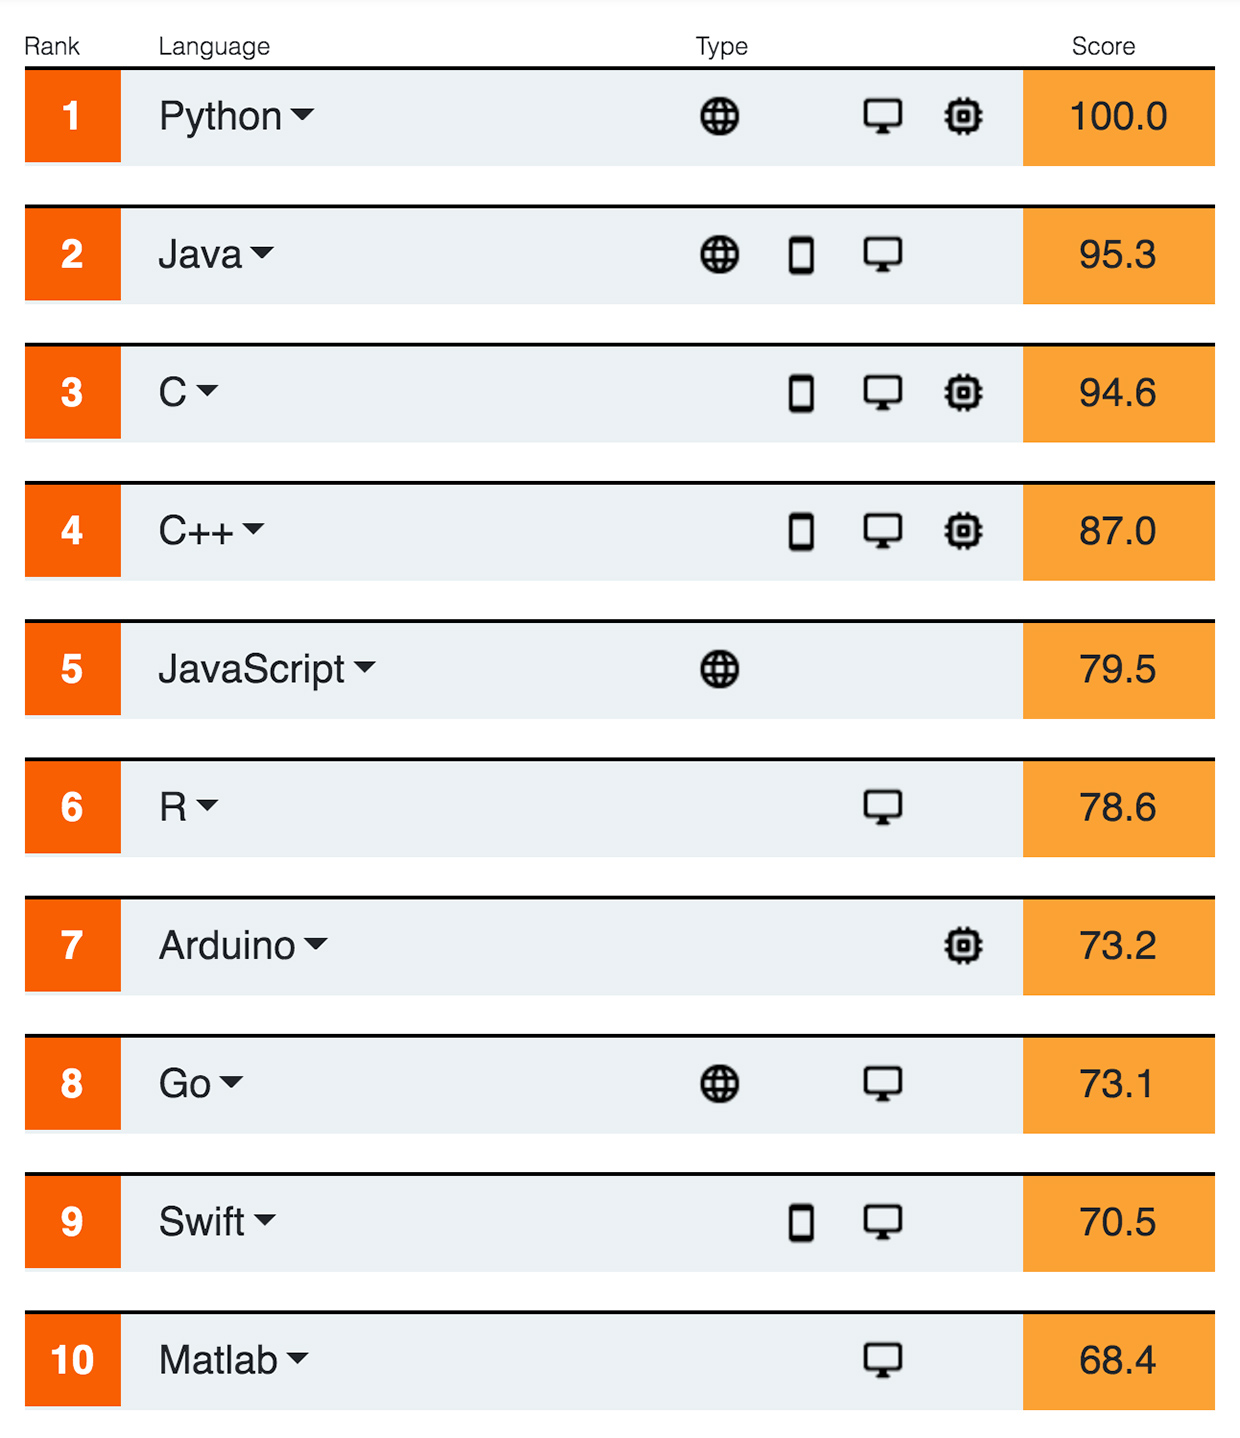
\includegraphics[scale=0.25]{./figures/cap2/ranking_python.jpeg}
	\caption{Linguagens de programação mais usadas em 2020}
\end{figure}

Outro ponto positivo de se usar Python é a replicabilidade, é possível criar painéis que atendam as diferentes Varas da JFRN, mostrando os dados que os gestores preferirem e acharem que são mais relevantes para suas realidades.

\section{Estrutura básica do painel}

Com os dados da JFRN em mãos e a ferramenta escolhida, passou-se a pesquisar quais seriam as bibliotecas usadas, portanto, a estrutura ficou da seguinte forma:

\begin{figure}[h]
	\centering
	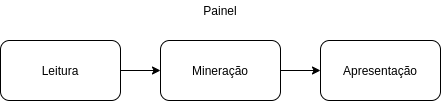
\includegraphics[scale=0.65]{./figures/cap2/estrutura_painel.png}
	\caption{Estrutura básica do painel}
\end{figure}

O painel que se propôs ao Centro de Inteligência não tem a estrutura clássica com diferentes tabelas (fato e dimensão), com as quais se geram as visualizações, no lugar disso, existe um arquivo .csv que contém os dados que serão usados, esses dados .csv fazem parte uma extração que veio do PJe, e a partir desse arquivo o painel vai criar subconjuntos de acordo com o ano e órgão julgador escolhidos pelo usuário. Portanto, esse painel se aproxima mais de um visualizador de dados do que de um painel BI.

Nele é possível selecionar duas variáveis: o Órgão Julgador e o Ano. A partir dessas escolhas o sistema vai fatiar os dados recebidos e mostrará algumas análises. Essas análises são mostradas em forma de tabelas condicionais, que mudam as cores das células de acordo com a frequência de aparição dos Assuntos.

\subsection{Estrutura dos dados}

Nessa primeira versão do painel os dados virão de um arquivo .csv gerado a partir do Qlikview, que é o software de BI padrão da JF. Esse arquivo carrega várias colunas, entre elas podemos citar número do processo, status, classe judicial, documento da parte, data do trânsito em julgado. Porém, para fazer a análise dos dados serão usadas as seguintes colunas:

\begin{itemize}
	\item Órgão Julgador - os órgão julgadores são as Varas da JFRN que ficam espalhadas pelo Estado, o usuário precisa selecionar um desses órgãos para visualizar os dados.
	
	\item Data Primeira Distribuição - essa é a data em que o processo chega na JFRN, mesmo que caia numa Vara que não seja da competência dele essa data é importante para analisar que Vara o recebeu e quando ele chegou na JFRN.
	
	\item Assunto - é o tema do processo, existem diferentes categorias em que um processo pode ser categorizado, e a partir desse campo é possível contar quantos processos de cada tipo deram entrada na JFRN.
	
	\item Assunto Código - diferentes assuntos possuem diferentes códigos, e a contagem dos processos se dá usando esse campo, que agrupa os códigos que são iguais e conta o total para saber quantos deram entrada na JFRN.
\end{itemize} 

A partir da escolha do Ano e do Órgão Julgador, o painel irá fazer as análises e seleções relevantes, populando a tabela e mostrando ao usuário quais são os processos mais frequentes de cada mês, no Ano e Vara escolhidos.

\subsection{Análise de anomalias}

A detecção de anomalias é, basicamente, uma técnica (ou um conjunto de técnicas) que servem para identificar comportamentos que fogem do que é esperado. Um dos desafios do trabalho foi encontrar uma forma de se detectar os Assuntos que possuíssem alta frequência de entrada na JFRN, porque, teoricamente, cada Ano e cada Vara possuem diferentes distribuições de probabilidade, e um modelo de detecção de anomalia que se encaixa bem em um determinado período, pode não se encaixar em outros. São 15 órgãos julgadores diferentes, e os anos que podem ser consultados são de 2014 até 2020, então são 90 distribuições diferentes. Portanto, usamos uma abordagem simples mas eficaz.

Primeiro, há uma análise da média ($\overline{x}$) de Assuntos que entraram na Vara, essa análise leva em conta o ano selecionado e o ano anterior, após isso, o desvio padrão ($\sigma$) é calculado e novas variáveis são geradas.

As variáveis são:
\begin{itemize}
	\item $anom_2$ que é a média mais duas vezes o desvio padrão, definida como: $$anom_2 = \overline{x} + 2*\sigma$$
	
	\item $anom_1$ que é a média mais uma vez o desvio padrão, definida como: $$anom_1 = \overline{x} + \sigma$$
	
	\item $media_{assuntos}$ que é a média simples dos assuntos, a cada dois anos:
	$$media_{assuntos} = \sum\limits_{ano}^{ano-1}\frac{assuntos}{total_{meses}}$$
\end{itemize}

Com essas variáveis encontradas, a distribuição das cores segue as regras a seguir, em que $total$ significa a quantidade total de Assuntos de determinada categoria:

\begin{equation}
	F_{cores} =
	\begin{cases}
		Vermelho & \text{se $total \geq anom_2$}\\
		Amarelo & \text{se $total \geq anom_1 \;e\; total < anom_2$}\\
		Verde & \text{se $total \geq media_{assuntos} \;e\; total < anom_1$}
	\end{cases}       
\end{equation}

\section{Bibliotecas usadas}

